\documentclass[11pt,a4paper]{jsarticle}
%
\usepackage[dvipdfmx]{graphicx}
\usepackage{here}
\usepackage{amsmath,amssymb}
\usepackage{bm}
\usepackage{graphicx}
\usepackage{ascmac}
\usepackage{listings,jvlisting}
%
\setlength{\textwidth}{\fullwidth}
\setlength{\textheight}{40\baselineskip}
\addtolength{\textheight}{\topskip}
\setlength{\voffset}{-0.2in}
\setlength{\topmargin}{0pt}
\setlength{\headheight}{0pt}
\setlength{\headsep}{0pt}
%
\newcommand{\divergence}{\mathrm{div}\,}  %ダイバージェンス
\newcommand{\grad}{\mathrm{grad}\,}  %グラディエント
\newcommand{\rot}{\mathrm{rot}\,}  %ローテーション
%
\lstset{
  basicstyle={\ttfamily},
  identifierstyle={\small},
  commentstyle={\smallitshape},
  keywordstyle={\small\bfseries},
  ndkeywordstyle={\small},
  stringstyle={\small\ttfamily},
  frame={tb},
  breaklines=true,
  columns=[l]{fullflexible},
  numbers=left,
  xrightmargin=0zw,
  xleftmargin=3zw,
  numberstyle={\scriptsize},
  stepnumber=1,
  numbersep=1zw,
  lineskip=-0.5ex
}
%
\title{システムソフトウェア 課題1}
\author{21B30362 佐久川泰輔}
\date{\today}
\begin{document}
\maketitle
%
%
\section{問1}

\subsection{コードの説明}
以下は、作成したpingpong.cのメイン関数の中身である。
\begin{lstlisting}[caption=pingpong.c]
int main(int argc, char *argv[]) {
    if (argc != 2) {
        fprintf(1, "usage: %s N\n", argv[0]);
        exit(1);
    }

    // # of rounds
    int n = atoi(argv[1]);

    // tick value before starting rounds
    int start_tick = uptime();

    int pp[2],qq[2];
    unsigned char buf[1];
    unsigned int num =0;

    //create pipe
    pipe(pp); //child -> parent
    pipe(qq); //parent -> child

    int status;
    if(fork() >  0){
        //parent process
        close(qq[0]);
        close(pp[1]);

        for(int i=0;i<n;i++){
            buf[0]=(unsigned char)num%256;
            write(qq[1],buf,1);
            read(pp[0],buf,1);
            num = (int)buf[0];
            num++;
        }

        //wait child process
        wait(&status);

        // tick value after ending rounds
        int end_tick = uptime();
        // print # of ticks in N rounds
        printf("# of ticks in %d rounds: %d\n", n, end_tick - start_tick);
        exit(0);
    }else{
        //child process
        close(pp[0]);
        close(qq[1]);

        for(int i=0;i<n;i++){
            read(qq[0],buf,1);
            num = (int)buf[0];
            num++;
            buf[0]=(unsigned char)num%256;
            write(pp[1],buf,1);
        }
    }
    exit(0);
}
\end{lstlisting}

まず、11行目でパイプを作成する前に開始時のティック数を記録する。

次に、親プロセスと子プロセスの間で通信を行うためのパイプを作成する。
ただし、パイプppは子プロセスから親プロセスの、パイプqqはその逆を行うために使用する。

その後、22行目でfork()を実行し、子プロセスを生成する。

23行目から42行目は親プロセスの処理を行うコードである。
27行目から33行目で、n回読み書きを行う。この際、書いた後に読むようにする。

44行目から54行目は子プロセスの処理を行うコードである。
48行目から54行目で、親プロせうと同様に読み書きを行う。この際、親プロセスとは逆に読んだ後に書くようにする。

親プロセスでは最後に、子プロセスの終了を待った後に終了時のティック数を記録する。

また、データの送信には要素数1のunsigned char型の配列を使用しているが、別プロセスからのデータを読み込んだ際は、これをunsigned int型にキャストし(28、52行目)、書き込む際にもキャストしている(31、50行目)。この際、unsigned intからunsigned charにキャストする時には、データがオーバーフローしないように256で割った後にキャストしている。


\subsection{実行結果}
実行結果は以下である。

\begin{figure}[H]
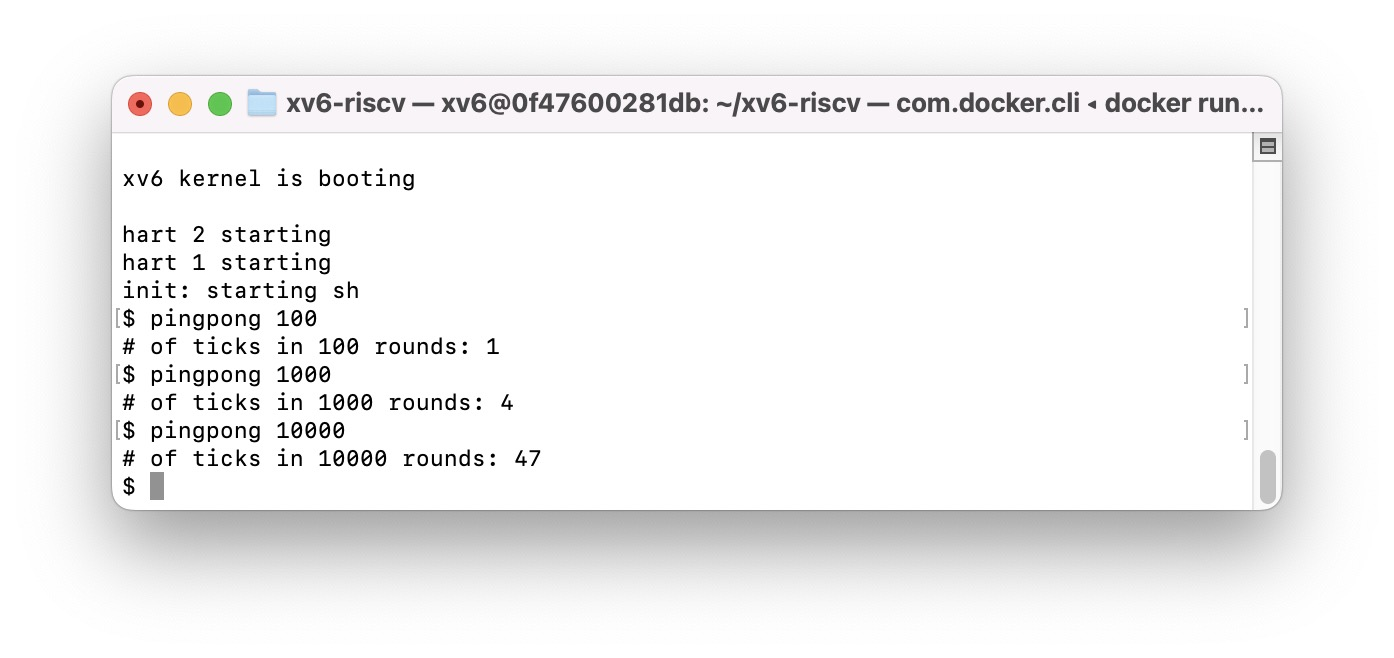
\includegraphics[width=0.8\linewidth]{image/figure1.png}
\end{figure}


\section{参考文献}
プロセス間通信について、以下のWebサイトを参考にした。

親プロセス・子プロセス間通信. https://qiita.com/penkopenko/items/f28d0b5ef404afd339fa. 2023-11-5
%
%
\end{document}